\section{Activity Diagram}

The Activity Diagram in Fig.~\ref{fig:activity-diagram} represents the main workflows of the Supplier Consumer Platform (SCP), showing how users interact with the system based on their company type and role. It outlines both consumer and supplier operations, as well as general chat and authentication flows.

\begin{figure*}[t]
\centering
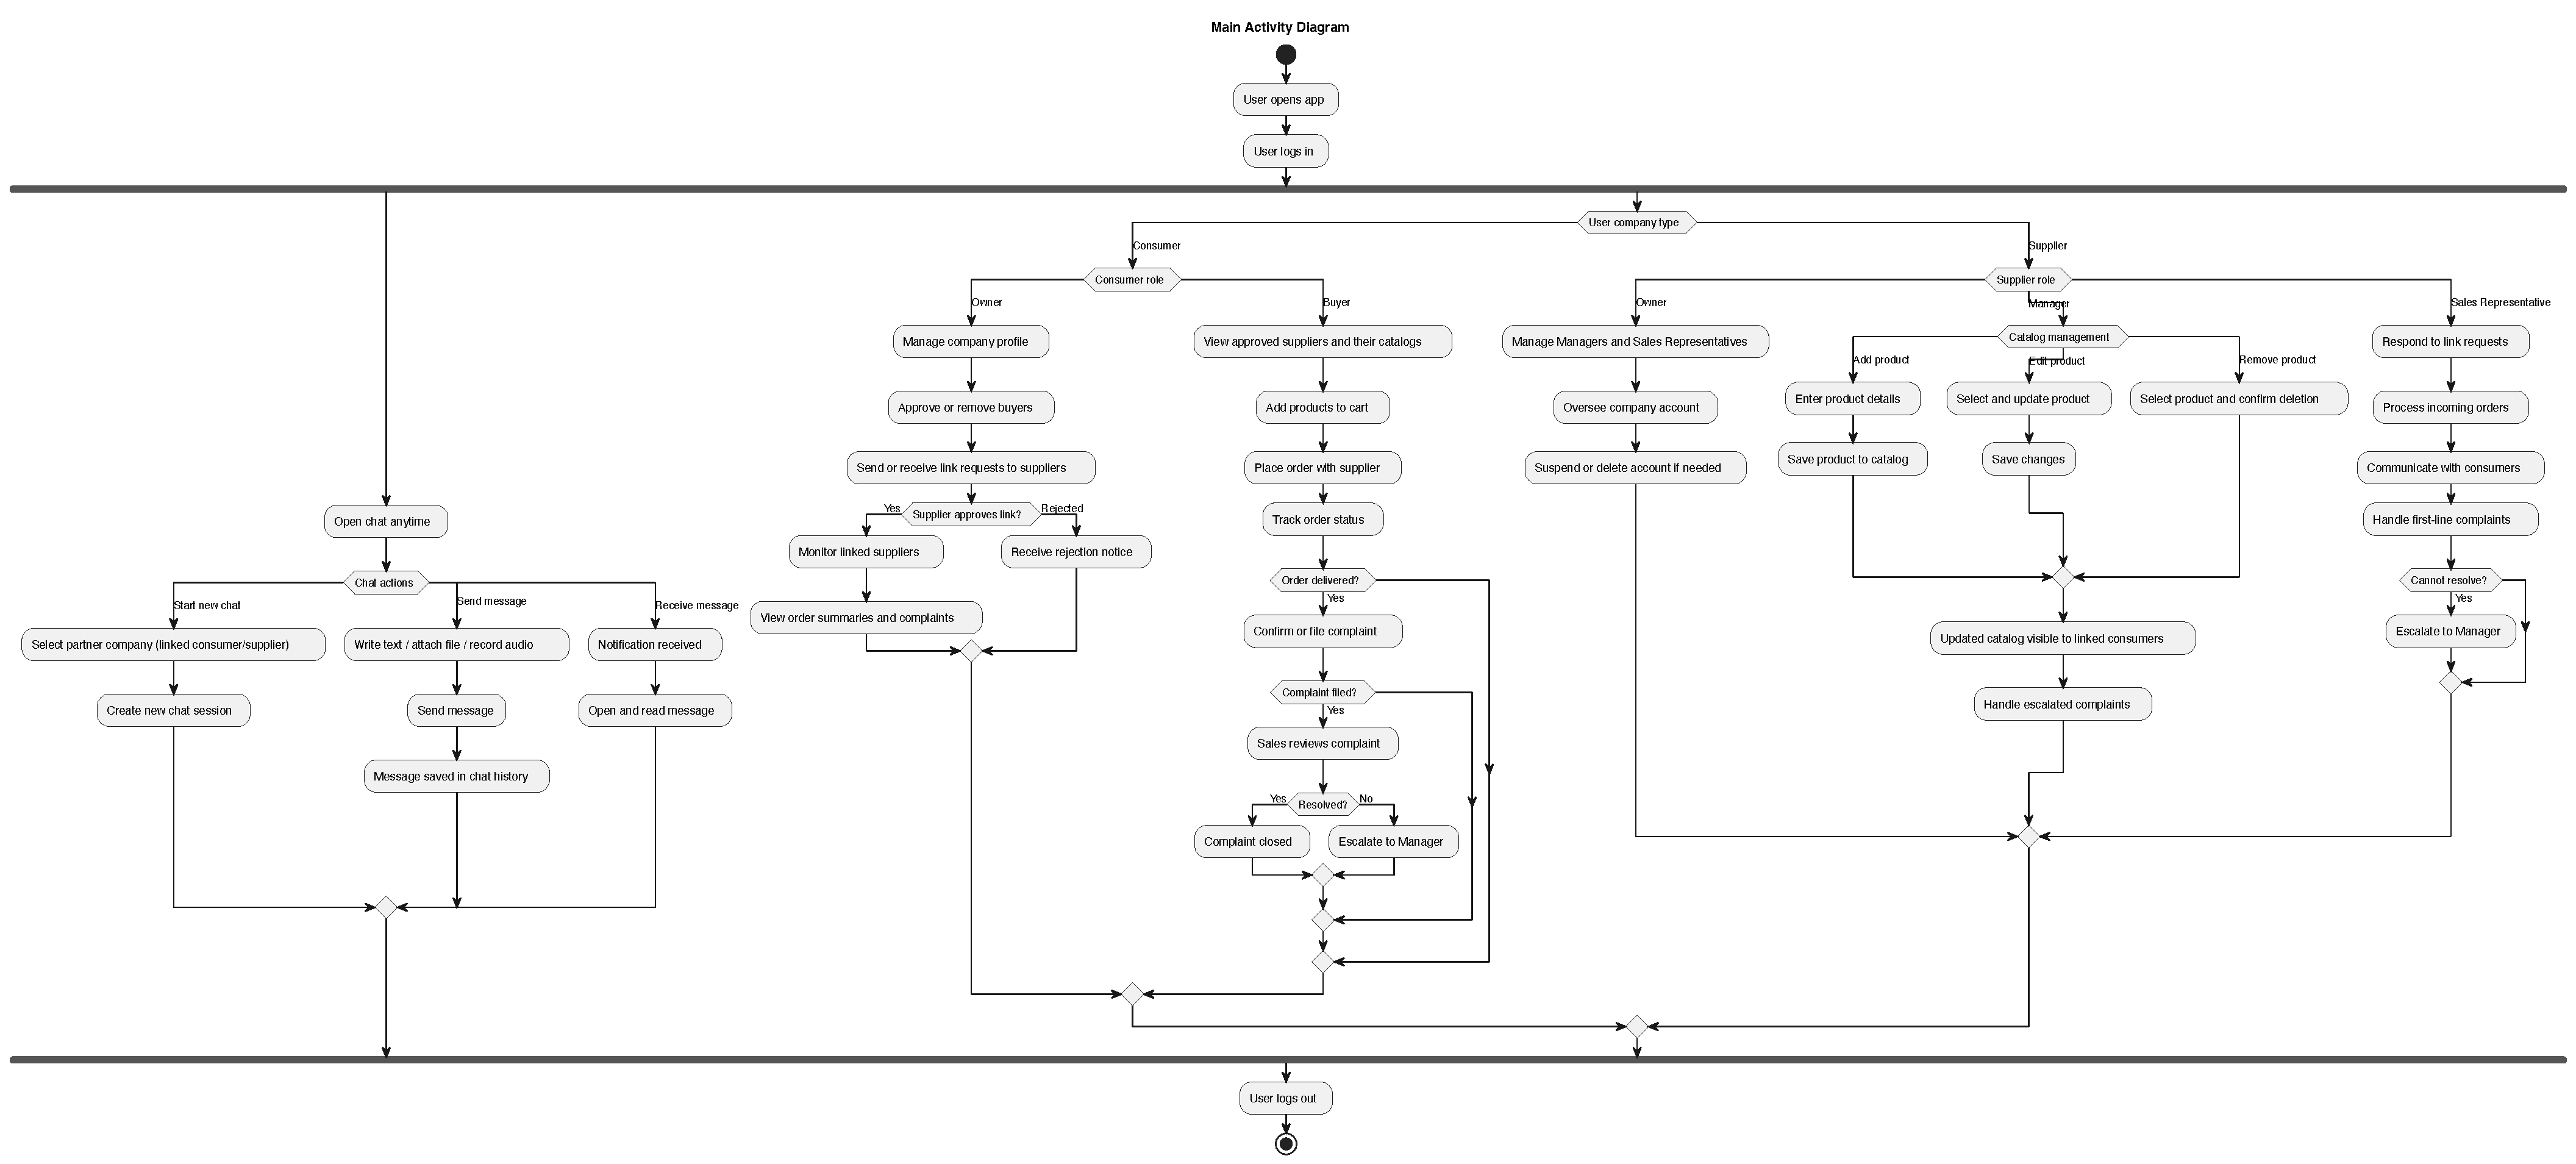
\includegraphics[width=0.9\textwidth]{out/main-activity-diagram.pdf}
\caption{Main Activity Diagram illustrating user interactions and workflows for Consumers and Suppliers.}
\label{fig:activity-diagram}
\end{figure*}

\subsection{Overview}

The diagram begins with the user launching the application and logging in. From this point, users can perform parallel activities through two primary branches:
\begin{itemize}
    \item General actions such as chatting and communication.
    \item Role-specific activities based on company type and assigned role.
\end{itemize}

This parallelism allows users to communicate through the in-app chat system while simultaneously performing business operations like managing orders, catalogs, or company staff.

\subsection{Consumer Flow}

For consumers, the activity diagram distinguishes between two roles: \textbf{Owner} and \textbf{Buyer}.

\begin{itemize}
    \item \textbf{Consumer Owner:} Responsible for managing the company profile, approving or removing buyer staff, and sending or receiving link requests to suppliers. Once a supplier approves the request, the owner can monitor linked suppliers and view order summaries and complaints.
    \item \textbf{Consumer Buyer:} Focuses on viewing approved suppliers, browsing their product catalogs, placing orders, and tracking order statuses. After an order is delivered, buyers can confirm delivery or file a complaint, which initiates the complaint handling process.
\end{itemize}

The complaint handling includes escalation paths: if a sales representative cannot resolve a complaint, it is forwarded to the supplier’s manager for final resolution.

\subsection{Supplier Flow}

For suppliers, the flow is divided among three roles: \textbf{Owner}, \textbf{Manager}, and \textbf{Sales Representative}.

\begin{itemize}
    \item \textbf{Supplier Owner:} Oversees the entire company account, manages managers and sales staff, and can suspend or delete the company account when necessary.
    \item \textbf{Supplier Manager:} Handles catalog management, including adding, editing, or removing products. Managers also address escalated complaints from sales representatives.
    \item \textbf{Sales Representative:} Manages incoming orders, responds to link requests, and handles first-level complaints. Unresolved issues are escalated to the manager.
\end{itemize}

All catalog changes made by managers become visible to linked consumers, ensuring synchronization of product information between suppliers and consumers.

\subsection{Chat Flow}

The chat subsystem operates independently and is accessible to all user types. Users can:
\begin{itemize}
    \item Initiate new chat sessions with linked partners.
    \item Send messages, files, or voice recordings.
    \item Receive and view notifications.
\end{itemize}

Each message is stored in chat history, ensuring traceability of communication between consumers and suppliers.

\subsection{End of Flow}

The process concludes when the user logs out, marking the termination of active sessions and parallel activities.

\section{Sequence Diagram}

The Sequence Diagram in Fig.~\ref{fig:sequence-diagram} captures the dynamic interactions among users, the application interface, and backend services. It presents the order of operations within several key workflows: staff management, linking, catalog management, order processing, and complaint handling.

\begin{figure*}[t]
\centering
\includegraphics[width=0.95\textwidth]{out/sequence-diagram.pdf}
\caption{Sequence Diagram showing interaction flows between user roles, the application, and backend services.}
\label{fig:sequence-diagram}
\end{figure*}

\subsection{Overview}

The diagram involves multiple user roles—Supplier Owner, Supplier Manager, Sales Representative, Consumer Owner, and Consumer Buyer—each interacting through the \textbf{Web/Mobile Application}. All requests are processed through a central \textbf{Backend API}, which communicates with various microservices such as the Company, User, Product, Order, Complaint, and Chat Services.

\subsection{Staff Management Flow}

Both Supplier and Consumer Owners can manage company staff via the User Service:
\begin{itemize}
    \item Retrieve existing staff lists.
    \item Add new staff members such as Managers, Sales Representatives, or Buyer staff.
\end{itemize}
The application sends user creation requests (\texttt{POST /users}) through the API, which delegates the operation to the User Service. Successful responses are displayed in the interface, confirming the creation of new staff accounts.

\subsection{Linking Flow}

The linking process allows Consumers and Suppliers to establish business connections:
\begin{itemize}
    \item The Consumer Owner initiates a link request through the Linking Service.
    \item The Supplier Owner reviews and either approves or rejects the request.
\end{itemize}
When approved, the API notifies both parties and automatically creates a shared chat session between them. This enables immediate communication for order and complaint handling.

\subsection{Catalog Management Flow}

Supplier Managers can manage product catalogs through the Product Service:
\begin{itemize}
    \item Add or edit product details.
    \item Update stock quantities.
\end{itemize}
Each modification is synchronized through API endpoints such as \texttt{POST /products} or \texttt{PATCH /products/\{id\}/stock}. Updated catalogs are then made visible to linked consumers.

\subsection{Order Flow}

The order workflow connects Consumer Buyers with Supplier Sales Representatives:
\begin{itemize}
    \item Consumers browse supplier catalogs and place orders.
    \item The Order Service verifies stock availability and confirms order creation.
    \item Sales Representatives view and accept incoming orders.
\end{itemize}
Notifications are exchanged between both parties to ensure real-time updates on order statuses.

\subsection{Complaint Flow}

The Complaint Service handles disputes or product issues:
\begin{itemize}
    \item Buyers can file complaints linked to specific orders.
    \item Sales Representatives first attempt resolution.
    \item If unresolved, the issue is escalated to the Supplier Manager.
\end{itemize}
The service tracks each complaint’s status (e.g., \texttt{pending}, \texttt{in\_progress}, \texttt{resolved}) and notifies the buyer once resolve_
